\chapter{Softwareumsetzung}
\label{cha:Software}

Mit Hilfe des in Kapitel \ref{sec:Kamera} beschriebenen Kameramoduls müssen verschiedene Aufgaben aus dem Bereich der Bildverarbeitung bewältigt werden. 

\section{Wahl der Bildverarbeitungsbibliothek}

Die Umsetzung der zu bewältigenden Aufgaben kann durch die Wahl einer geeigneten Bildverarbeitungsbibliothek deutlich vereinfacht werden. Wichtige Kriterien für die Wahl der Bibliothek sind unter anderem Funktionsumfang, Dokumentation und Aktivität der Community.

\subsection{LibCCV}

LibCCV \cite{libccv} ist eine open-source Bildverarbeitungsbibliothek, die viele bekannte Algorithmen implementiert. LibCCV steht unter einer BSD-Clause-3-Lizenz und kann somit für eine Studienarbeit problemlos unbegrenzt verwendet werden. Die Bibliothek ist größtenteils in C++ verfasst und somit potenziell auf einem Android-Smartphone verwendet werden. Die Verwendung auf dem Smartphone wird jedoch nicht offiziell unterstützt und kann potenziell weitere Schwierigkeiten mit sich bringen.

\subsection{Imagemagick}

Bei Imagemagick \cite{imagemagick} handelt es sich um eine Bildverarbeitungsbibliothek, welche sehr viele Algorithmen bereits implementiert hat. Algorithmen zur Objekterkennung müssten jedoch vollständig selbst implementiert werden, was zu einem großen zusätzlichen Aufwand führen kann. Imagemagick wird unter der Apache 2.0 Lizenz vertrieben.

\subsection{OpenCV}
\label{subsec:opencv}

OpenCV \cite{opencv_library, bradski2008learning} stellt eine der größten Open-Source-Bibliotheken für Bildverarbeitung da. Die Bibliothek hat einen starken Fokus auf Echtzeitverarbeitung und wird daher auch in vielen Projekten im Bereich der Robotik verwendet. OpenCV hat eine große aktive Community, wodurch eventuelle Fragen und Probleme schnell beantwortet werden können. Zusätzlich bietet OpenCV eine offizielle Version für Android und eignet sich somit ideal für diese Studienarbeit.


\section{Algorithmen zur Objekterkennung}
\label{sec:Objekterkennung}

Aufgabe des Roboters, ist es Gegenstände in einem Raum mit Hilfe von Kamerabildern zu erkennen. Folglich spielt die Objekterkennung eine große Rolle.

\subsection{Farbbasierte Objekterkennung}
Einen einfachen Ansatz der Objekterkennung unter Verwendung von Methoden der in \ref{subsec:opencv} beschriebenen Bibliothek OpenCV stellt eine farbbasierte Objekterkennung dar. Hierfür wird das Kamerabild zunächst vom RGB-Format in das HSV-Format konvertiert. Dies wird durchgeführt, da das HSV-Format unempfindlicher gegen Veränderungen in der Beleuchtung ist als das RGB-Format \cite{cucchiara2001improving}. Abbildung \ref{fig:ColorModels} zeigt die Aufteilung eines Bildes in die verschiedenen Kanäle.

\begin{figure}[h]
\centering
\includegraphics[width=\textwidth]{Bilder/Software/ColormodelsAll}
\caption{Beispiel einer Aufspaltung in RGB-Kanäle (links) und HSV-Kanäle (rechts)}
\label{fig:ColorModels}
\end{figure}

Wie in Abbildung \ref{fig:ColorModels} zu sehen ist, eignet sich vor allem der Saturation-Kanal des Bildes um farbige Objekte zu erkennen, da dieser hohe Werte annimmt wenn die Farbintensität hoch ist. Zuletzt erfolgt eine Binarisierung mit einem empirisch ermittelten Schwellwert von 50. Dies ist notwendig, da die, in der OpenCV-Bibliothek implementierte, Methode von Suzuki und Abe \cite{suzuki1985topological} zur Segmentierung von Objekten ein Binärbild erwartet. Aus dem in Abbildung \ref{fig:ColorModels} dargestellten Beispiel entsteht nach der Binarisierung schließlich Abbildung \ref{fig:BinarizedColorModels}. Der Algorithmus zur Segmentierung erkennt daraus drei Objekte und zeichnet ihren Konturen, wie in Abbildung \ref{fig:SegmentedColorModels} ersichtlich, ein.

\begin{figure}[h]
\centering
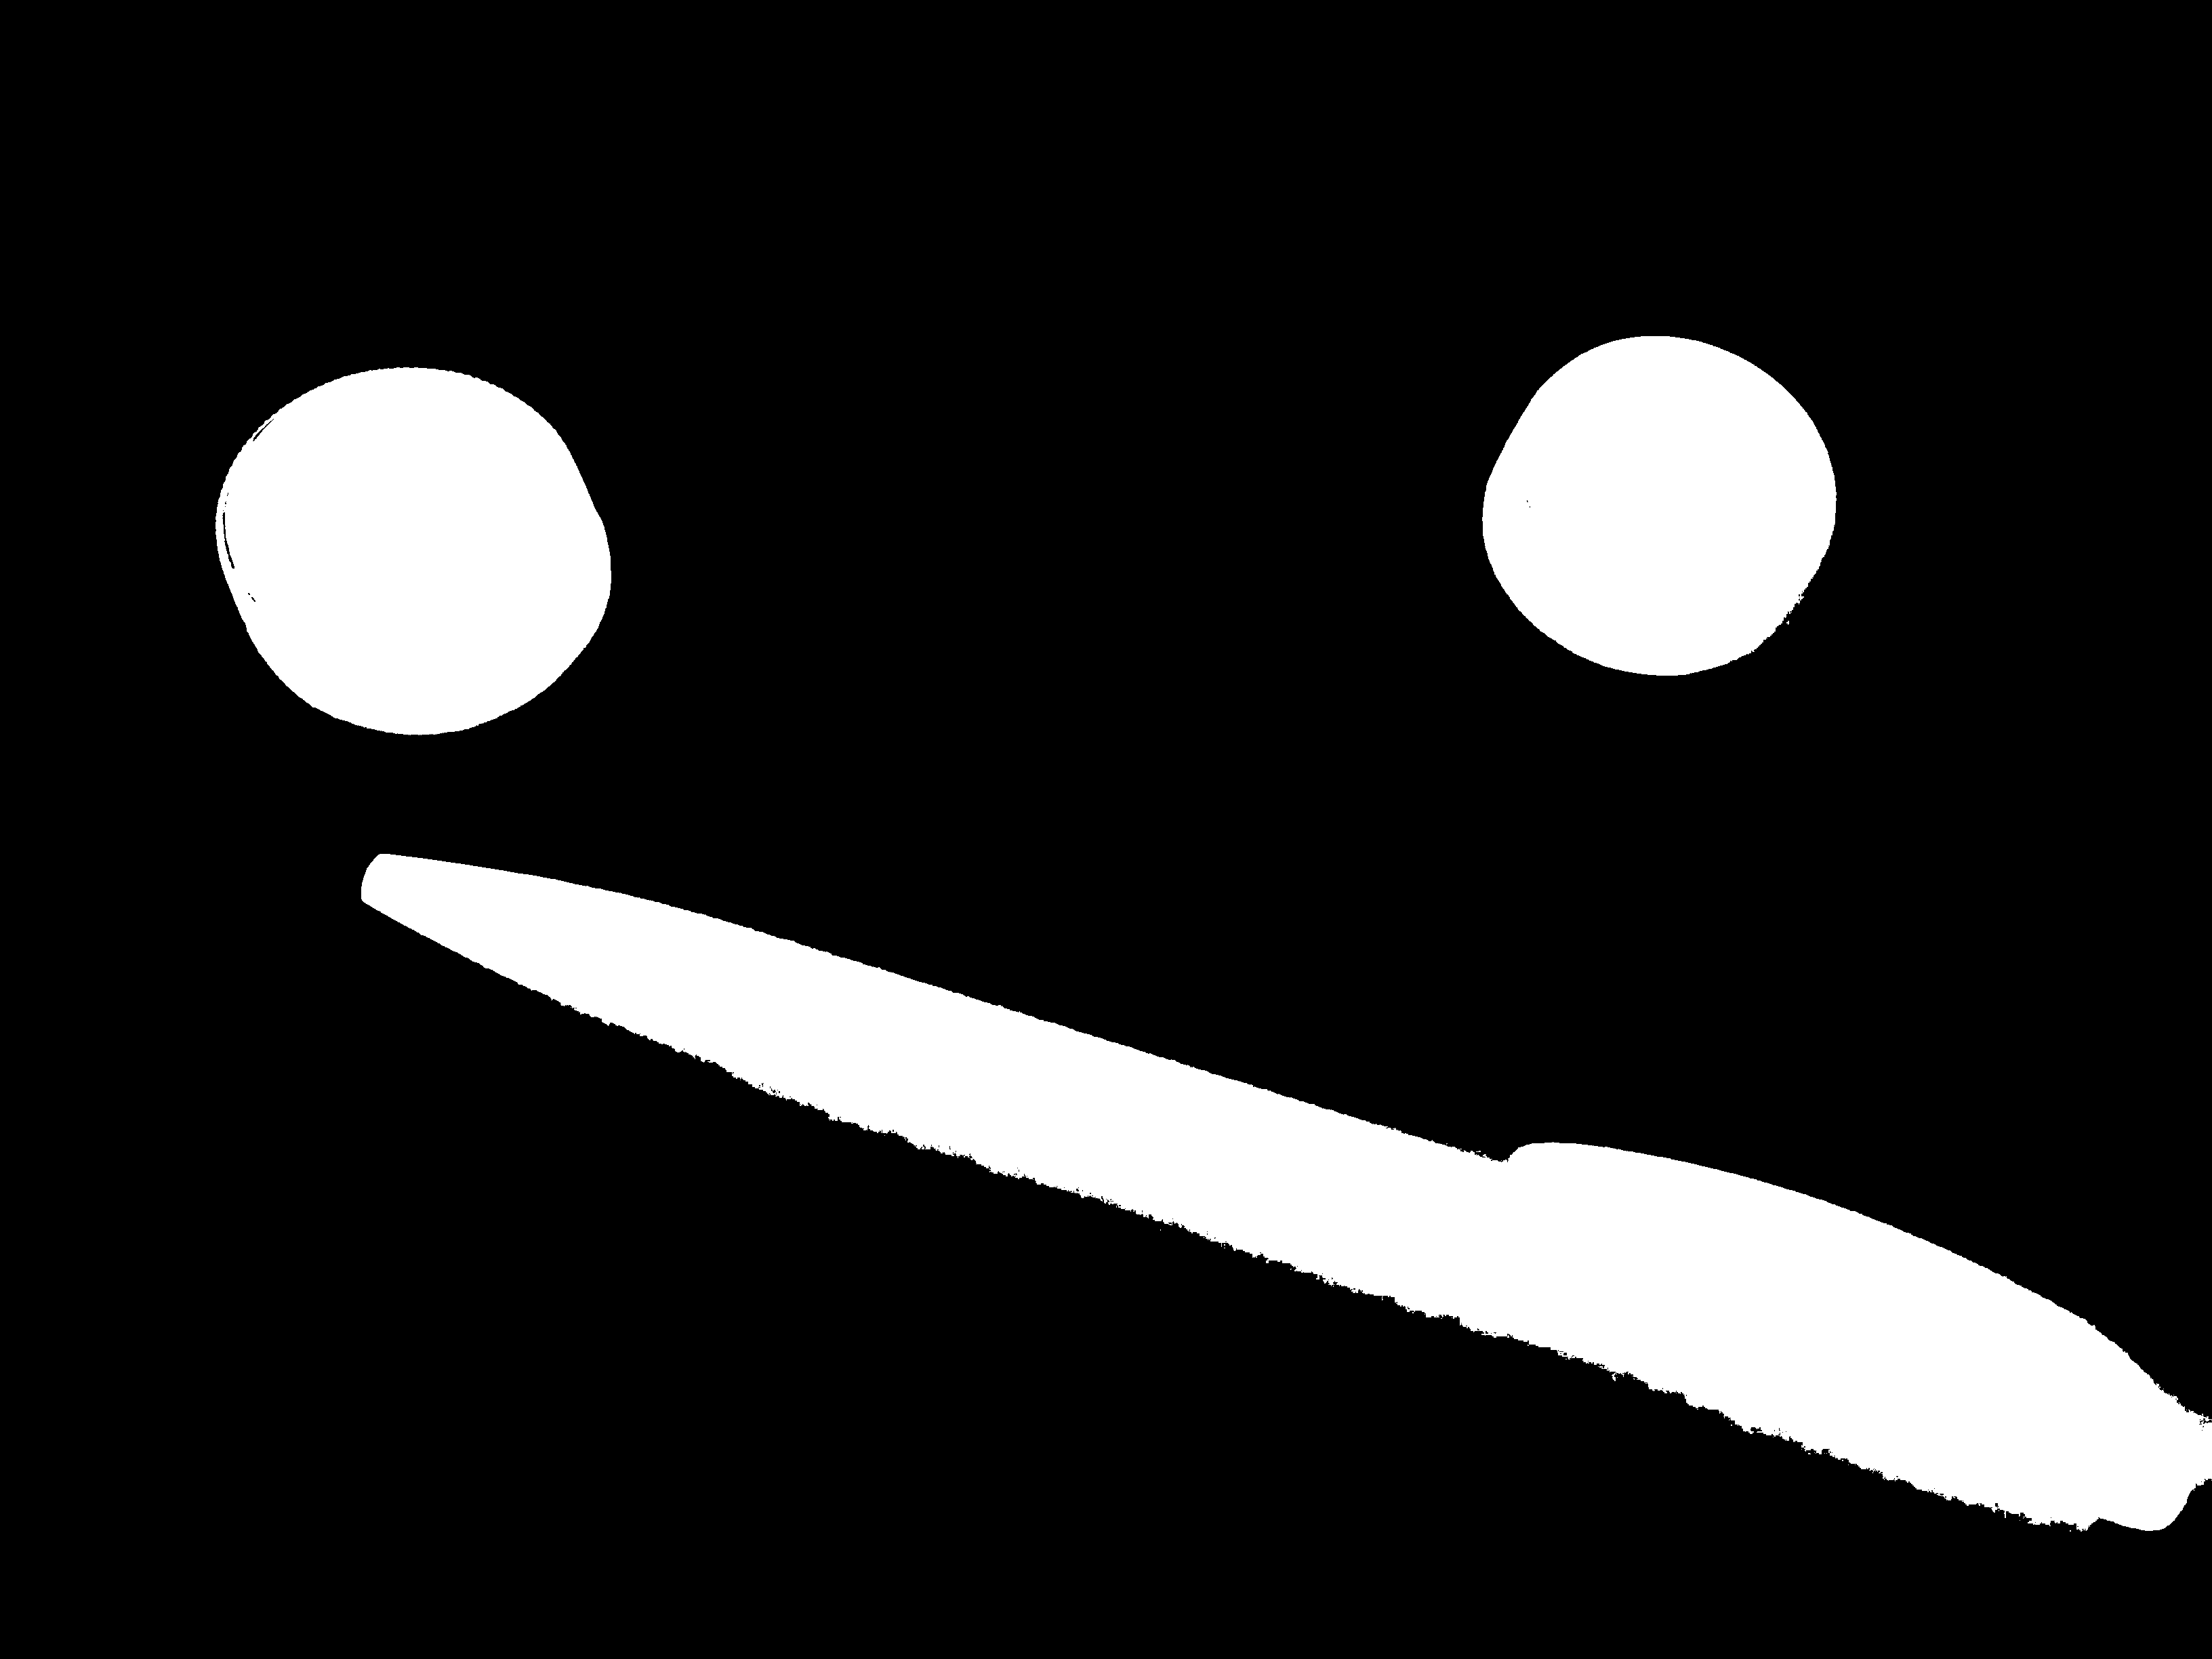
\includegraphics[width=\textwidth/2]{Bilder/Software/ColormodelsBinarized}
\caption{Beispiel der Binarisierung des Sättigungskanals}
\label{fig:BinarizedColorModels}
\end{figure}
\begin{figure}[h]
\centering
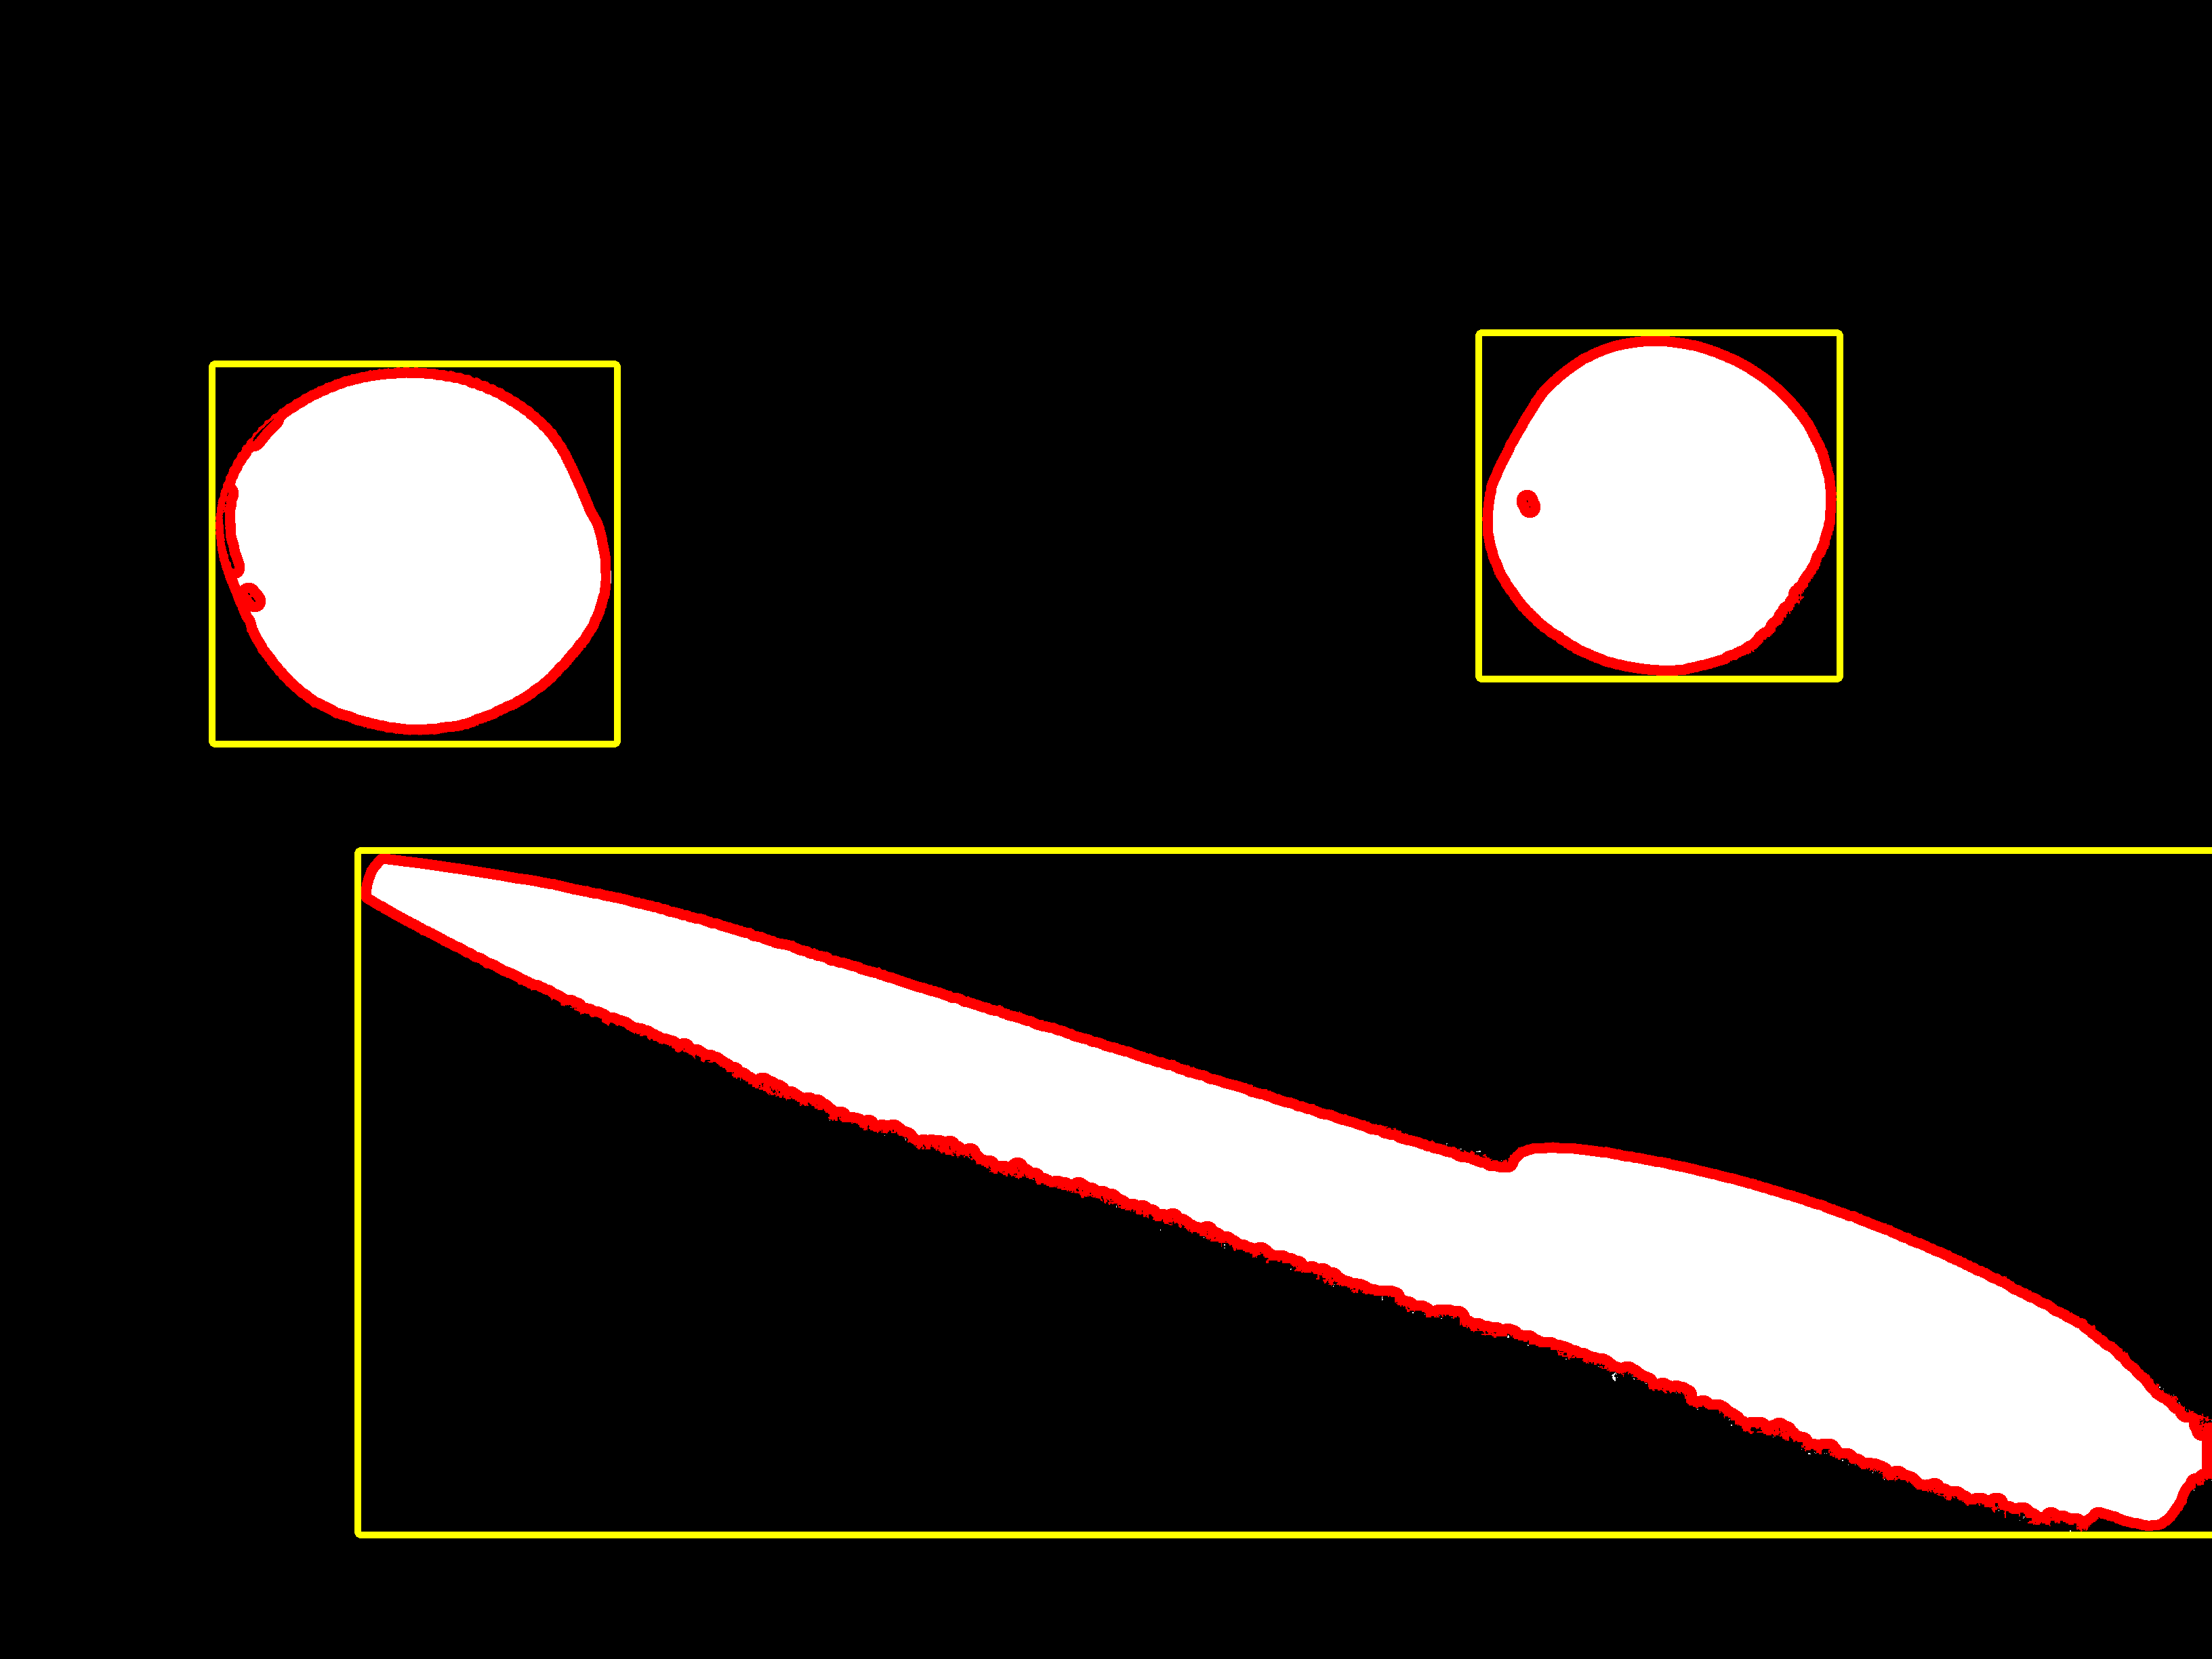
\includegraphics[width=\textwidth/2]{Bilder/Software/ColormodelsSegmentated}
\caption{Beispiel einer Segmentierung des binarisierten Sättigungskanals}
\label{fig:SegmentedColorModels}
\end{figure}

\section{Ortsbestimmung}
\label{sec:Ortsbestimmung}

Die Aufgabe des Roboters ist es, Gegenstände in vordefinierte Bereiche zu befördern. Hierzu muss ihm jederzeit bekannt sein wo diese sich befinden, bzw. wo er sich relativ zu diesen aufhält, um sie anfahren zu können.

\subsection{Mitteilung von Beobachterkomponente}
\label{subsec:Beobachter}

Ist im Raum ein weiteres System vorhanden, dessen Position konstant und dem Roboter zu jedem Zeitpunkt bekannt ist, kann eine simple, und genaue Positionsbestimmung erfolgen. Eine solche Beobachterkomponente kann über Sensordaten, wie beispielsweise einer Kamera oder einem Ultraschallsensor, zu jedem Zeitpunkt Kontakt zu Roboter haben.
Der Roboter muss hierbei keine Berechnungen durchführen und verlässt sich für die korrekte Positionsbestimmung auf den Beobachter, von welchem zu jedem Zeitpunkt Position und Orientierung des Roboters im Raum abrufbar ist.

Die Beobachterkomponente stellt eine sehr effiziente Art von Ortsbestimmung dar, hat jedoch den beträchtlichen Nachteil, dass zusätzliche Hardware erforderlich ist.

\subsection{Raumanalyse}

Bei der Raumanalyse werden Kamerabilder analysiert und aus ihnen Fixpunkte oder Geraden extrahiert, mit denen sich der Roboter bei Bewegung im Raum zu orientieren versucht. Dies ist ein sehr rechenaufwändiges Verfahren, welches zusätzlich mit einer großen Implementierungsarbeit verbunden ist.

Zusätzlich stellt dieses Verfahren Anforderungen an den Raum in dem es verwendet wird. Im Raum müssen genügend charakteristische Orientierungspunkte vorhanden sein. Verliert der Roboter die Orientierung, ist es nicht ohne weiteres möglich diese wiederzuerlangen.

Vorteil des Verfahrens der Raumanalyse ist, dass die benötigte Hardware in Form eines Kameramoduls und eines leistungsstarken Prozessors bereits vorhanden ist.

\subsection{Positionsverfolgung}

Die Positionsverfolgung als Mittel der Ortsbestimmung bietet sich bei Robotern an, welche einen sehr exakten Sensor zur Beobachtung der zurückgelegten Strecke besitzen. Über die zurückgelegte Strecke und die Orientierung des Roboters kann zu jedem Zeitpunkt ein Bewegungsvektor erzeugt werden, der die genaue Position des Roboters bestimmt.

Problematisch bei diesem Verfahren ist jedoch, dass eine sehr genaue Bestimmung der zurückgelegten Strecke benötigt wird. Fehler bei der Bestimmung wirken sich additiv aus. Die hat zur Folge, dass die Positionsverfolgung bei längeren Fahrten immer ungenauer wird. Eine Art der Streckenbestimmung stellen beispielsweise Rotationssensoren in Rädern dar. Hierbei wird die Genauigkeit des Verfahrens durch das Spiel der Räder und der Auflösung der Sensoren beeinträchtigt.

Da das CLEEN-R-Projekt nicht über die zusätzliche Hardware einer Beobachterkomponenten verfügt und der zusätzliche Aufwand der Auswertung der Kamerabilder zur Merkmalsextraktion zu aufwändig wäre, wurde sich für die Variante der Positionsverfolgung entschieden. Die Auflösung der Rotationssensoren ist mit 1\degree\ ausreichend genau. Die automatische Geschwindigkeitsanpassung der NXT-Motoren abhängig des Untergrunds fördern zusätzlich eine exakte Ortsbestimmung über die Positionsverfolgung.

\section{Struktur der Applikation}
Da es sich um eine große Applikation mit mehr als 3000 Zeilen Code und 33 Klassen handelt, sind in den folgenden Abschnitten lediglich Kernelemente herausgegriffen und im Detail erklärt.

\subsection{Grundstruktur}
Eine Android Applikation muss mindestens eine Klasse haben, die von der abstrakten Klasse \textit{Activity} erbt. Diese Activity, oftmals \textit{MainActivity} genannt, wird beim Starten der Applikation aufgerufen. Sie verwaltet grafische Oberflächen, sowie das Verhalten der Applikation beim Starten, Schließen oder Pausieren. Im CLEEN-R-Projekt stellt die \textit{MainActivity} zusätzlich eine Schnittstelle zur OpenCV-Bibliothek dar. Die Activity wird über eingehende Kamerabilder informiert und vermittelt diese weiter an den Controller der Applikation; die Klasse \textit{CleenrBrain}.

Zusätzlich hält die \textit{MainActivity} eine Referenz zur Klasse der Hardwareansteuerung \textit{NxtTalker}. Abbildung \ref{fig:UMLActivity} zeigt die Grundstruktur der \textit{MainActivity}

\begin{figure}[H]
\centering
\scalebox{.4}{
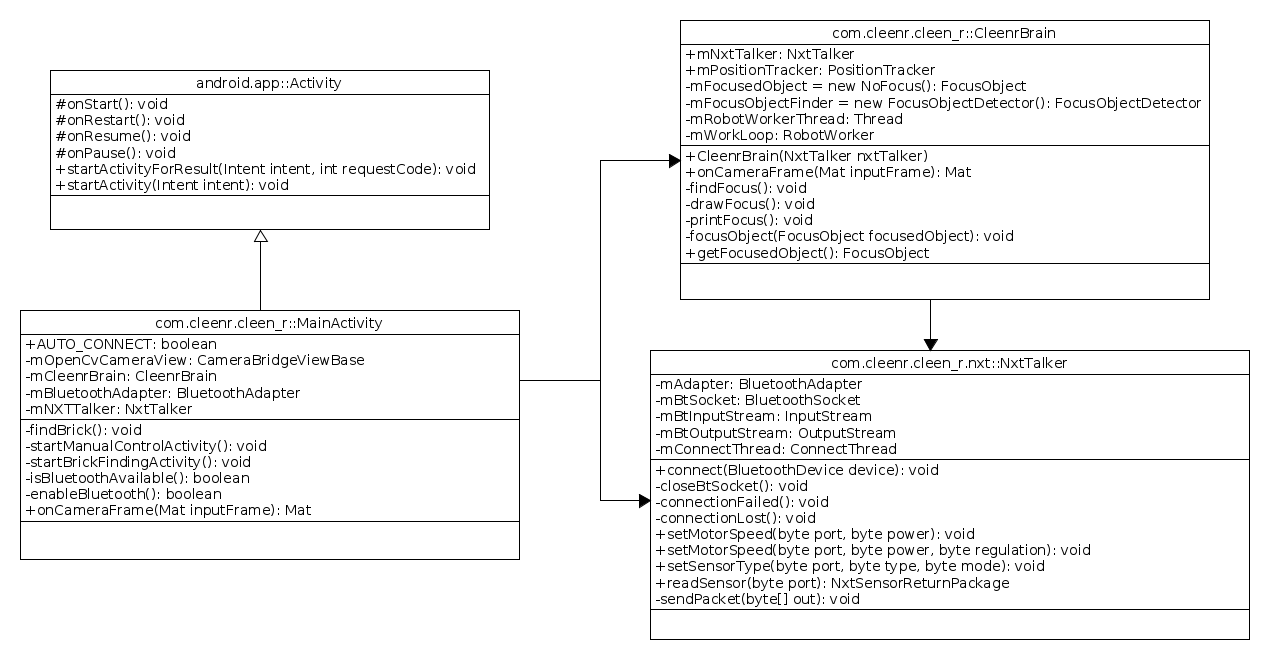
\includegraphics{Bilder/Software/UML/MainActivity}
}
\caption{UML-Klassendiagramm der Grundstruktur der Applikation}
\label{fig:UMLActivity}
\end{figure}

 
\subsection{Fokusobjektfindung}

Die Controllerklasse \textit{CleenrBrain} hat die Aufgabe den Roboter zu koordinieren. \textit{CleenrBrain} hält eine Referenz zu einem \textit{FocusObject}-Objekt, welches den aktuell fokussierten Gegenstand repräsentiert. Hierbei wird auch das Fehlen eines Fokusobjekts aus Gründen der Polymorphie als Objekt beschrieben. \textit{CleenrBrain} wird beim vorliegen einer neuen Kameraaufnahme benachrichtigt und ermittelt daraufhin mit Hilfe einer \textit{FocusObjectDetector}-Klasse ein neues \textit{FocusObject}. Hierbei wird, wie in Kapitel \ref{subsec:Auffindung} beschrieben versucht einen Gegenstand über mehrere Aufnahmen hinweg im Fokus zu behalten. Abbildung \ref{fig:UMLFocus} beschreibt das Zusammenspiel der beschriebenen Klassen anschaulich.

\begin{figure}[H]
\centering
\scalebox{.4}{
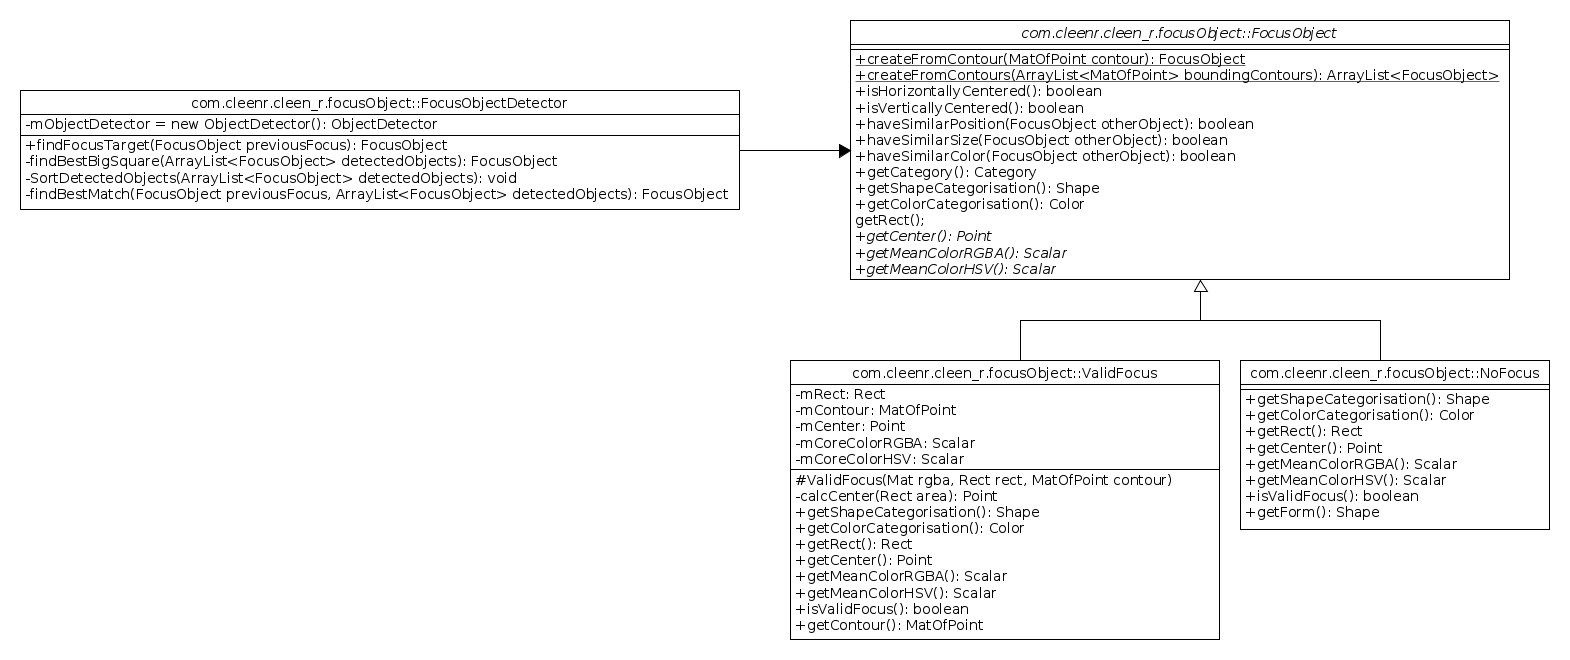
\includegraphics{Bilder/Software/UML/FocusObjects}
}
\caption{UML-Klassendiagramm der für die Auffindung eines Fokusobjekts verantwortlichen Klassen}
\label{fig:UMLFocus}
\end{figure}

\subsection{Objektkategorisierung}

Wie auch aus Abbildung \ref{fig:UMLFocus} ersichtlich, beinhaltet die \textit{FocusObject}-Klasse eine Methode zur Kategorisierung des Gegenstands. Hierbei wird eine Kategorie der Klasse \textit{Category} erzeugt, welche sich aus den beiden Feldern \textit{Color} und \textit{Shape} zusammensetzt.

\begin{figure}[H]
\centering
\scalebox{.4}{
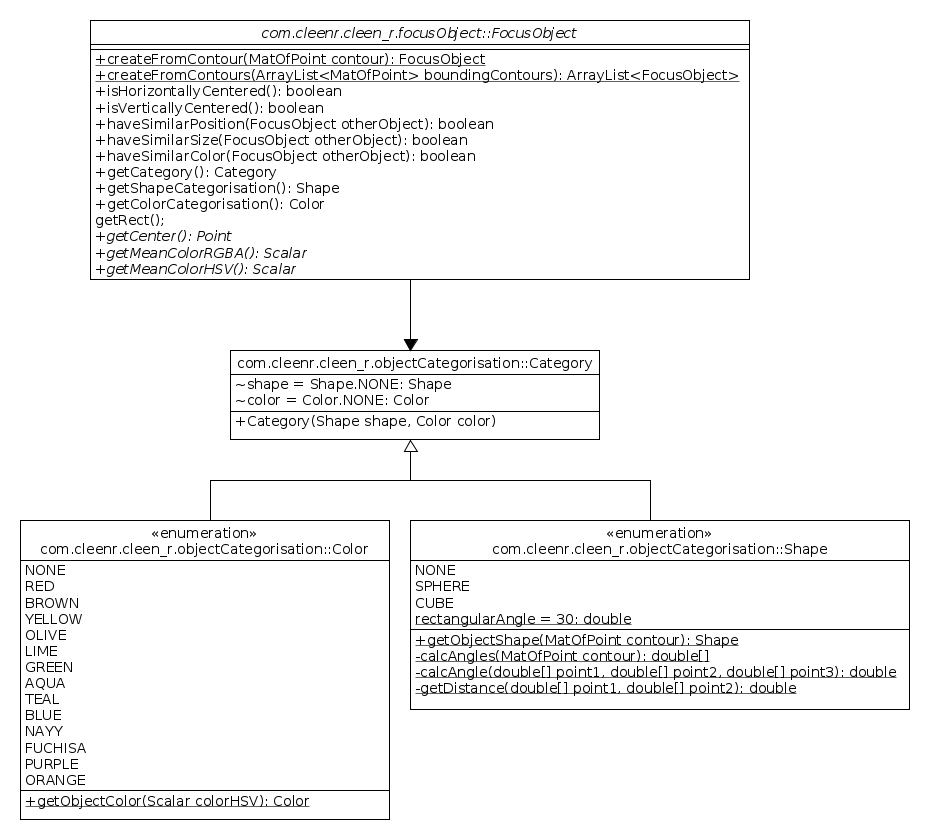
\includegraphics{Bilder/Software/UML/Categories}
}
\caption{UML-Klassendiagramm der Kategorisierung von Fokus Objekten}
\label{fig:UMLCategorisation}
\end{figure}

\subsection{Bewegungssteuerung und Positionsverfolgung}

Die Bluetooth-Verbindung wird mittels einer \textit{NxtTalker}-Instanz durch einen Aufruf von \textit{MainActivity} aus initiiert. Ein Thread überwacht den Stream auf eingehende Sensordaten und setzt Befehle an den NXT ab.

Bewegungsbefehle der Workloop gehen in die Klasse \textit{NxtControlUnit} ein, von wo aus sie von \textit{NxtTalker} in Bluetooth-Befehle übersetzt werden. Die Verfolgung der Roboterposition wird hauptsächlich in der Klasse \textit{PositionTracker} abgewickelt. Jeder Bewegungsbefehl setzt eine Mitteilung an \textit{PositionTracker} ab, welcher dann anhand Dauer und Geschwindigkeit der Bewegung die neuen Koordinaten berechnet.

\begin{figure}[H]
\centering
\scalebox{.4}{
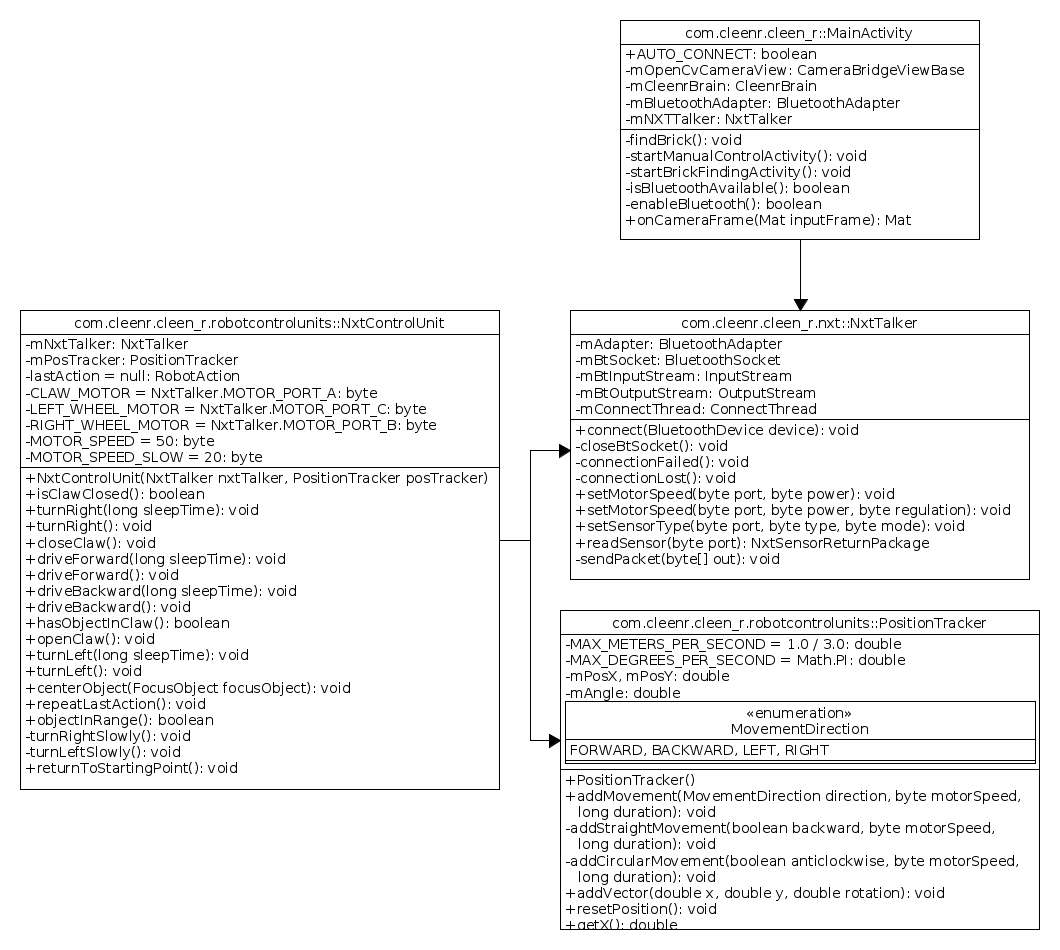
\includegraphics{Bilder/Software/UML/Movement}
}
\caption{UML-Klassendiagramm der Bewegungssteuerung und Positionsverfolgung}
\label{fig:UMLMovement}
\end{figure}

\subsection{Arbeitsphasen}

Die Controllerklasse \textit{CleenrBrain} verwaltet mit Hilfe eines zusätzlichen Threads den Arbeitszyklus des Roboters. Durch die Verwendung eines zweiten Threads kann die Suche nach neuen Fokus Objekten in folgenden Aufnahmen parallel zur Abarbeitung der in Kapitel \ref{cha:Workloop} beschriebenen Arbeitsphasen geschehen. 

Die Arbeitsphasen sind separat als eigene Klassen modelliert, die sich von einer abstrakten Klasse \textit{WorkPhase} ableiten. Jede Arbeitsphase verfügt über eine virtuelle \textit{executeWork}-Methode, welche Zugriff auf alle für die Arbeitsphase relevanten Operationen besitzt. Darunter zählen Steuerwerk des Roboters, eine Referenz auf das aktuelle Fokusobjekt und einer Möglichkeit die Arbeitsphase zu wechseln. Die Implementierung der \textit{PickingUpObject}-Klasse ist in Listing \ref{lst:Pickup} erkennbar. Es ist deutlich zu sehen, dass der Code durch die hinzugefügte Abstraktionsebene sehr einfach gehalten werden kann.

\begin{lstlisting}[caption={Implementierung der Arbeitsphase \glqq Gegenstand aufnehmen\grqq }, label=lst:Pickup]
public class PickingUpObject extends WorkPhase {
    public PickingUpObject(RobotWorker worker) {
        super(worker);
    }
    @Override
    public void executeWork(FocusObject focusObject, RobotControlUnit controlUnit) {
        controlUnit.closeClaw();
        if (!controlUnit.hasObjectInClaw()) {
            controlUnit.openClaw();
            mRobotWorker.switchWorkphase(new SearchingObject(mRobotWorker));
            return;
        }
        mRobotWorker.switchWorkphase(new CategorisingObject(mRobotWorker));
    }
}
\end{lstlisting}

